\subsection{OTFS Receiver Design}

The receiver of the baseline OTFS system performs the inverse operation of the transmitter front-end. After the transmitted waveform passes through the time-varying multipath channel, the received time-domain signal is first converted back to the time-frequency domain and then transformed to the delay-Doppler domain. The resulting delay-Doppler symbols are not directly used for hard symbol decisions. Instead, they form the observation vector for the message passing detector described in Section 3.6.

In the simulation model, the receiver processing contains two main operations: the Wigner transform and the symplectic finite Fourier transform (SFFT). The Wigner transform converts the received time-domain samples into a time-frequency grid, while the SFFT converts the time-frequency grid back to the delay-Doppler domain.

\subsubsection{Overview of the Receiver Processing Chain}

The receiver starts from the sampled received signal \(\mathbf{r}\), which includes the effect of the doubly dispersive channel and additive noise. This signal is reshaped into a two-dimensional matrix so that the receiver can process it over the same \(M \times N\) OTFS frame structure used at the transmitter. The first transform extracts the received time-frequency symbols. The second transform maps these symbols back into the delay-Doppler domain.

\begin{figure}[H]
    \centering
    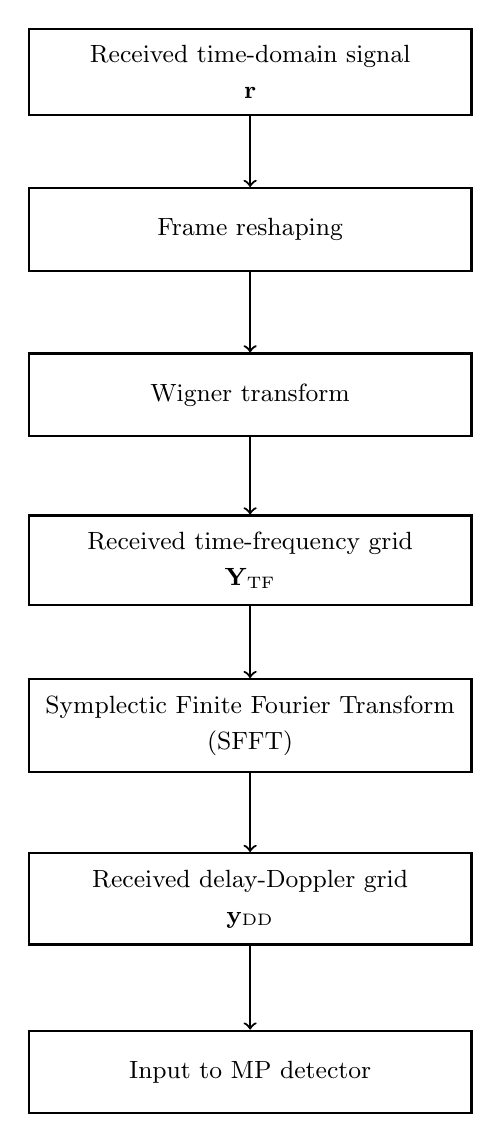
\begin{tikzpicture}[
        block/.style={
            rectangle,
            draw,
            thick,
            align=center,
            text width=5.2cm,
            minimum height=1.05cm,
            font=\small,
            inner sep=6pt
        },
        arrow/.style={
            ->,
            thick,
            shorten >=0pt,
            shorten <=0pt
        }
    ]

        \node[block] (rx) at (0,0) {Received time-domain signal\\[2pt]\(\mathbf{r}\)};
        \node[block] (reshape) at (0,-2.0) {Frame reshaping};
        \node[block] (wigner) at (0,-4.1) {Wigner transform};
        \node[block] (tf) at (0,-6.2) {Received time-frequency grid\\[2pt]\(\mathbf{Y}_{\mathrm{TF}}\)};
        \node[block] (sfft) at (0,-8.3) {Symplectic Finite Fourier Transform\\[2pt](SFFT)};
        \node[block] (dd) at (0,-10.5) {Received delay-Doppler grid\\[2pt]\(\mathbf{y}_{\mathrm{DD}}\)};
        \node[block] (detector) at (0,-12.7) {Input to MP detector};

        \draw[arrow] (rx.south) -- (reshape.north);
        \draw[arrow] (reshape.south) -- (wigner.north);
        \draw[arrow] (wigner.south) -- (tf.north);
        \draw[arrow] (tf.south) -- (sfft.north);
        \draw[arrow] (sfft.south) -- (dd.north);
        \draw[arrow] (dd.south) -- (detector.north);

    \end{tikzpicture}
    \caption{Baseline OTFS receiver processing chain}
    \label{fig:otfs_receiver_chain}
\end{figure}

Figure~\ref{fig:otfs_receiver_chain} shows that the receiver does not directly demodulate QAM symbols after the SFFT stage. This is important because the time-varying channel causes coupling among delay-Doppler symbols. Therefore, the receiver front-end only reconstructs the received delay-Doppler observation, while the actual symbol estimation is performed later by the detector.

\subsubsection{Received Signal Reshaping}

Let \(\mathbf{r}\) denote the received time-domain sample vector after the channel. This vector is reshaped into an \(M \times N\) matrix as

\begin{equation}
    \mathbf{R} = \mathrm{reshape}(\mathbf{r}, M, N).
\end{equation}

This operation restores the frame structure before applying the receiver transforms. It is the counterpart of the serialization step at the transmitter, where the time-domain transmit matrix is converted into a one-dimensional signal vector.

The reshaping operation itself does not remove channel distortion or noise. It only prepares the received samples for the Wigner transform.

\subsubsection{Wigner Transform}

The Wigner transform is used to convert the received time-domain samples into the time-frequency domain. In the discrete implementation, this operation is performed by an \(M\)-point FFT along the delay-related dimension of the reshaped received signal. The resulting time-frequency grid is denoted by \(\mathbf{Y}_{\mathrm{TF}}\).

In matrix form, the discrete Wigner stage can be represented as
\begin{equation}
    \mathbf{Y}_{\mathrm{TF}}
    =
    \left(
    \frac{1}{\sqrt{M}}\mathbf{F}_{M}\mathbf{R}
    \right)^{T},
    \label{eq:receiver_wigner_matrix}
\end{equation}
where \(\mathbf{F}_{M}\) denotes the \(M\)-point DFT matrix. The transpose follows the grid-index convention used by the transmitter-side time-frequency matrix.

The normalization factor \(\sqrt{M}\) is used to keep the signal energy consistently scaled with the transmitter implementation. After the FFT, the transpose operation arranges the matrix so that the received time-frequency samples follow the same indexing convention as the transmitted grid \(\mathbf{X}_{\mathrm{TF}}\).

Conceptually, this stage can be interpreted as the receiver counterpart of the Heisenberg transform. While the Heisenberg transform generates the time-domain waveform from the time-frequency grid, the Wigner transform extracts the time-frequency representation from the received waveform.

\subsubsection{Symplectic Finite Fourier Transform}

After obtaining the received time-frequency grid, the receiver applies the SFFT to map the signal back to the delay-Doppler domain. This is the inverse operation of the ISFFT used at the transmitter. If \(Y[n,m]\) denotes the received time-frequency sample, the corresponding delay-Doppler observation \(y[k,l]\) is obtained as

\begin{equation}
    y[k,l]
    =
    \frac{1}{\sqrt{MN}}
    \sum_{n=0}^{N-1}
    \sum_{m=0}^{M-1}
    Y[n,m]
    e^{-j2\pi\left(\frac{nk}{N}-\frac{ml}{M}\right)} .
\end{equation}

This equation is the most important receiver-side transform in the baseline OTFS model. It explains how the received signal is returned to the delay-Doppler domain, where the channel has a sparse and structured representation.

In discrete matrix processing, the SFFT combines one Fourier operation and one inverse Fourier operation along the two OTFS grid dimensions. The normalization term is selected consistently with the transmitter-side ISFFT normalization, ensuring that the overall modulation and demodulation chain has compatible energy scaling.

\subsubsection{Received Delay-Doppler Observation}

The output of the OTFS demodulator is the received delay-Doppler grid \(\mathbf{y}_{\mathrm{DD}}\). In an ideal channel without noise or Doppler-delay spreading, this grid would match the transmitted delay-Doppler symbol grid. In the simulated doubly dispersive channel, however, each received grid point may contain contributions from several transmitted symbols due to delay shifts, Doppler shifts, and complex fading coefficients.

Therefore, the received delay-Doppler grid should be understood as an observation, not as a final decision. The receiver front-end produces

\begin{equation}
    \mathbf{y}_{\mathrm{DD}} = \mathrm{SFFT}\left\{\mathbf{Y}_{\mathrm{TF}}\right\},
\end{equation}

and this observation is then passed to the message passing detector. The detector uses the channel information, delay taps, Doppler taps, and path coefficients to estimate the transmitted QAM symbols.

This separation between demodulation and detection is important in OTFS. The demodulator only changes the signal representation, while the detector resolves the interference introduced by the time-varying multipath channel.

\subsubsection{Discrete Receiver Processing Summary}

The complete receiver front-end can be summarized by the ordered sequence
\begin{equation}
    \mathbf{r}
    \xrightarrow{\text{frame reshaping}}
    \mathbf{R}
    \xrightarrow{\text{Wigner transform}}
    \mathbf{Y}_{\mathrm{TF}}
    \xrightarrow{\text{SFFT}}
    \mathbf{y}_{\mathrm{DD}} .
    \label{eq:receiver_discrete_summary}
\end{equation}
The first operation restores the received OTFS frame. The Wigner transform then extracts the time-frequency grid, and the SFFT returns the observation to the delay-Doppler domain.

This processing order is consistent with the transmitter chain. The transmitter maps delay-Doppler symbols to the time-frequency domain using the ISFFT and then generates the time-domain signal using the Heisenberg transform. The receiver reverses this order by first applying the Wigner transform and then the SFFT.

\subsubsection{Summary of the Baseline OTFS Receiver}

The baseline OTFS receiver converts the received time-domain waveform back into a delay-Doppler observation through two main operations. The Wigner transform extracts the time-frequency grid from the received samples, and the SFFT maps this grid into the delay-Doppler domain. The receiver output is not yet the estimated transmitted data, because the delay-Doppler symbols are still affected by channel-induced interference.

The overall receiver front-end can be summarized as

\begin{equation}
    \mathbf{r}
    \rightarrow
    \mathbf{R}
    \rightarrow
    \mathbf{Y}_{\mathrm{TF}}
    \rightarrow
    \mathbf{y}_{\mathrm{DD}} .
\end{equation}

The delay-Doppler observation \(\mathbf{y}_{\mathrm{DD}}\) is then used as the input to the message passing detector. This completes the receiver-side signal transformation and prepares the system for symbol estimation, which is discussed in the following sections.
